\documentclass[dvipsnames]{beamer}

\addtobeamertemplate{navigation symbols}{}{%
    \usebeamerfont{footline}%
    \usebeamercolor[fg]{footline}%
    \hspace{1em}%
    \insertframenumber/\inserttotalframenumber
}

% Thème
\usetheme{Darmstadt}
\usecolortheme{seahorse}
\usepackage[T1]{fontenc}

%% La langue
\usepackage[english]{babel} 

% Math
\usepackage{bbm}
\usepackage{amsthm}
\usepackage{amsmath}
\usepackage{stmaryrd}
\usepackage{amssymb}
\usepackage{proof}
\usepackage{tikz}
\usepackage{booktabs}
\usetikzlibrary{positioning}
\newcommand{\mcl}{\mathcal{L}}
\newcommand{\mce}{\mathcal{E}}
\newcommand{\mcd}{\mathcal{D}}
\newcommand{\mcc}{\mathcal{C}}
\newcommand{\ra}{\rightarrow}
\newcommand{\rsa}{\rightsquigarrow}
\newcommand{\llb}{\llbracket}
\newcommand{\rrb}{\rrbracket}
\newcommand{\R}{\mathbb{R}}
\newcommand{\C}{\mathbb{C}}
\newcommand{\K}{\mathbb{K}}
\renewcommand{\S}{\mathbb{S}}
\newcommand{\tend}[1]{\underset{#1\to +\infty}{\longrightarrow}}

%inference
\usepackage{semantic}

% colors
\usepackage{xcolor}

% barrer
 \usepackage{soul}

% wrap images around text
\usepackage{wrapfig}

% listing (code)
\usepackage{listings}
\lstset{
 language=caml,
 columns=[c]fixed,
 basicstyle=\small\ttfamily,
 keywordstyle=\color{blue},
 commentstyle=\color{Green}\bfseries,
 breaklines=true,
 mathescape=true
}

\newcommand{\etat}[1]{\langle #1 \rangle}
\newcommand{\etatz}[1]{\langle #1 \rangle_0}
\newcommand{\etatu}[1]{\langle #1 \rangle_1}
\newcommand{\etatd}[1]{\langle #1 \rangle_2}
\newcommand{\etatt}[1]{\langle #1 \rangle_3}

\definecolor{blue2}{rgb}{0.7, 0.83, 1}
\definecolor{orange}{rgb}{1, 0.83, 0.7}
\definecolor{grey}{RGB}{200,200,200}
\definecolor{link_color}{RGB}{0,0,200}

% \setbeamercolor{palette primary}{bg=Tan!30,fg=black}
% \setbeamercolor{palette secondary}{bg=Tan!70,fg=black}
% \setbeamercolor{palette tertiary}{bg=Tan!70,fg=black}
% \setbeamercolor{palette quaternary}{bg=Tan!10,fg=black}

% % 1- Block title (background and text)
% \setbeamercolor{block title}{bg=Bittersweet!50,fg=black}
% % 2- Block body (background)
% \setbeamercolor{block body}{bg=Bittersweet!10}

% % 1- Block title (background and text)
% \setbeamercolor{block title alerted}{bg=RedViolet!70,fg=black}
% % 2- Block body (background)
% \setbeamercolor{block body alerted}{bg=RedViolet!10}

% % 1- Block title (background and text)
% \setbeamercolor{block title example}{bg=ForestGreen!70,fg=black}
% % 2- Block body (background)
% \setbeamercolor{block body example}{bg=ForestGreen!10}


% Titre
\title{Two models, two measures}
\author{Ewen DUFOUR}
\institute{Université Paris-Saclay\\
Laboratoire Méthodes Formelles}
\date{16 juillet 2025}
\AtBeginSection[]
{ \begin{frame}
    \frametitle{Outline}
    \tableofcontents[currentsection]
  \end{frame} }

% Document
\begin{document}
\frame{\titlepage}

\section{Introduction}
\begin{frame}{Internship environment.}
\end{frame}
\subsection*{Problem presentation}
\begin{frame}{Invariance thesis.}
  \begin{itemize}
    \item Presented by Slot and Van Emde Boas.
    \item Existence of a computation model class.
    \item Contains Turing machines, RAM, etc.
    \item Simulate each other with:
     \begin{itemize}
        \item Polynomial overhead in time.
        \item Linear overhead in space.
      \end{itemize}
  \end{itemize}
\end{frame}
\begin{frame}{$\lambda$-calculus complexity.}
  What about $\lambda$-calculus?
  \begin{itemize}
    \item Time:
      \pause
      \begin{itemize}
        \item Weak $\lambda$-calculus.\checkmark
          \pause
        \item Strong $\lambda$-calculus.\checkmark
      \end{itemize}
      \pause
    \item Space:
      \begin{itemize}
        \item Only partial solutions.
      \end{itemize}
  \end{itemize}
\end{frame}
\begin{frame}{Linear substitution calculus.}  
\begin{itemize}
  \item $t ::=~x~|~\lambda x.t~|~t~t~|~t[x/t]$
\item  $\mcl ::= \square~|~\mcl[x/t]$
  \item $\mcc ::= \square~|~\mcc[x/t]~|~t[x/\mcc]~|~\mcc~t~|~t~\mcc~|~\lambda x.\mcc$
  \item Reduction rules:
    \begin{itemize}
      \item $ \mcl[\lambda x.t]~u~\ra_{d\beta}~\mcl[t[x/u]] $
      \item $\mcc\llb x\rrb[x/u]~\ra_{ls}~\mcc\llb u\rrb[x/u]$
      \item  $t[x/u]~\ra_{gc}~t \quad x\notin fv(t)$
    \end{itemize}
\end{itemize}
\end{frame}
\begin{frame}{Attack plan.}
  \begin{center}
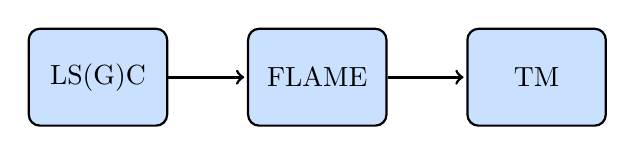
\begin{tikzpicture}[auto,
        every path/.style ={draw, ultra thick, ->, % -Stealth[],
                            shorten >=1pt, line width=1pt},
        every node/.style ={thick, align=center, rounded corners, rectangle, minimum height=3.5em, minimum width=5em},
        WorkedOn/.style  ={ draw=black,  fill=blue2!70},
    ]

% Nodes

\node (b) [WorkedOn] {FLAME};
\node (a) [WorkedOn, left=of b] {LS(G)C};
\node (c) [WorkedOn,right=of b] {TM};


% Arrows
\draw (a) -- (b);
\draw (b) -- (c);

\end{tikzpicture}
\end{center}
\end{frame}
\section{Definitions}
\subsection*{LS(G)C}
\begin{frame}{Terms and strategy.} 
  \pause
  \begin{block}{Values}
  We distinguish as values the terms given by the grammar: $v ::= \lambda x.t~|~v[x/t]$
  \end{block}
  \pause
  \begin{block}{Evaluation contexts}
  For our strategy, we will use the contexts given by the grammar: $\mcc ::= \square~|~\mcc[x/t]~|~\mcc~t~|~v~\mcc$  
\end{block}
\begin{block}{Remark}
 We are no more substituting under abstraction or explicit substitutions. 
\end{block}
\end{frame}
\begin{frame}{Terms and strategy.}
    \begin{block}{Reduction strategy} 
    \begin{align*}
    &\infer[LA]{t~u\rightarrow t'~u}{t \rightarrow t'}
 &\infer[RA]{v~t\rightarrow v~t'}{t \rightarrow t'}\\
&\infer[GC]{t[x/u]\rightarrow t'}{t \rightarrow t' & x \notin fv(t') }
&\infer[US]{t[x/u]\rightarrow t'[x/u]}{t \rightarrow t' & x \in fv(t')}\\
&\infer[LS]{\mathcal{C}\llbracket x \rrbracket [x/u]\rightarrow \mathcal{C}\llbracket u \rrbracket [x/u]}{x \in fv(\mathcal{C}\llbracket u \rrbracket) }
&\infer[LSGC]{\mathcal{C}\llbracket x \rrbracket [x/u]\rightarrow \mathcal{C}\llbracket u \rrbracket}{x \notin fv(\mathcal{C}\llbracket u \rrbracket) }\\
&\infer[DB]{\mathcal{L}[\lambda x.t]~v \rightarrow \mathcal{L}[t[x/v]]}{x\in fv(t)}
&\infer[DBGC]{\mathcal{L}[\lambda x.t]~v \rightarrow \mathcal{L}[t]}{x\notin fv(t)}
\end{align*}
  \end{block}
\end{frame}


\begin{frame}{Space cost.}
  \begin{alertblock}{Space function for terms}
    We define the space function $|~|$ on terms as following:
  \begin{align*}
    |x| &= |dB(x)|\\
    |\lambda x.t| &= 1 + |t|\\
    |t~u| &= |t|+|u|\\
    |t[x/u]| &= |t|+|u|
  \end{align*}
  We extend this definition to contexts.
  \end{alertblock}
  \begin{block}{Remark}
    We assume that the actual terms are represented with de Bruijn indices.
  \end{block}
\end{frame}

\subsection*{FLAME}
\begin{frame}{FLAME.}
\begin{itemize}
    \item Decompose the term.
    \item Do the reduction.
    \item Recompose the term.
      \item Do all again until it tries to reduce a value.
  \end{itemize} 
\end{frame}
\begin{frame}{Transitions.}
\begin{block}{FLAME transitions}
\label{FLAME}
\centering
\resizebox{\textwidth}{!}{%
\begin{tabular}{@{}l l l l l l l l l l@{}}
\toprule
\textbf{arg} & \textbf{term} & \textbf{context} & \textbf{state} & \textbf{transition}& \textbf{arg} & \textbf{term} & \textbf{context} & \textbf{state} \\
\midrule

– & $t[ u ] $ & $\mcc$ & 0 & $\rsa_{us}$ & – & $t$ & $\textsf{LS}(u) :: \mcc$ & 0  \\

- & $t~u$ & $\mcc$ & 0 & $\rsa_{lapp}$ & – & $t$ & $\textsf{RA}(u) ::\mcc$ & 0  \\
- & $v~t$ & $\mcc$ & 0 & $\rsa_{rapp}$ & – & $t$ & $\textsf{LA}(v) :: \mcc$ & 0  \\
- & $n$  & $\mcc$ & 0 & $\rsa_{ls}$ & - & $\uparrow^{n+1} t$ & $\mcc$ & 2 & $\textsf{LS}(t)=\textsf{nth\_subst}(\mcc)$ \\
- & $v_1~v_2$  & $\mcc$ & 0 & $\rsa_{db}$ & $(v_2,0)$ & $v_1$ & $\mcc$ & 1  \\

$(v_2, n)$ & $v_1[ t ]$ &$\mcc$ & 1 & $\rsa_{rdb}$ & $(v_2, n+1)$ & $v_1$ & $\textsf{LS}(t) :: \mcc$ & 1\\ 
$(v, n)$ & $\lambda.t $ &$\mcc$ & 1 & $\rsa_{fdb}$ & - & $t$ & $\textsf{LS}(\uparrow^{n}v) :: \mcc$ & 2 & $0\in fv(t)$\\
$(v, n)$ & $\lambda.t $ &$\mcc$ & 1 & $\rsa_{fdbgc}$ & - & $\downarrow t$ & $\mcc$ & 2& $0\notin fv(t)$\\
-&$v$ & $[]$ & 2 & $\rsa_{stop}$ & -& $v$ &$[]$ & 3 \\
-&$t$ & $[]$ & 2 & $\rsa_{dive}$ & -& $t$ &$[]$ & 0 \\
-&$t$ & $\textsf{LS}(u) :: \mcc$ & 2 & $\rsa_{gc}$ & -& $\downarrow t$ &$\mcc$ & 2 & $0\notin \textsf{fv}(t)$ \\
-&$t$ & $\textsf{LS}(u) :: \mcc$ & 2 & $\rsa_{bsubst}$ & -& $t[ u ]$ &$\mcc$ & 2 & $0\in \textsf{fv}(t)$ \\
-&$t$ & $\textsf{RA}(u) :: \mcc$ & 2 & $\rsa_{blapp}$ & -& $t~u$ &$\mcc$ & 2 \\
-&$t$ & $\textsf{LA}(u) :: \mcc$ & 2 & $\rsa_{brapp}$ & -& $u~t$ &$\mcc$ & 2 \\

% \bottomrule
\end{tabular}
}
% \caption{FLAME transitions.}
\end{block}
\end{frame}
\begin{frame}{Cost model.}
  \begin{block}{Notation}
    An actual state of the machine is given by $\etat{(v,n),t,\mcc}_e$. %where
    % \begin{itemize}
    %   \item $t$ is the term we are evaluating.
    %   \item $\mcc$ is a pile of contexts.
    %   \item $(v,n)$ is a possibly empty couple where $v$ is the argument of an application and $n$ is the distance to the abstraction;
    % \end{itemize}
  \end{block}
  \begin{alertblock}{Space function for states.}
  We define the space function $|~|$ on states as following:
  \begin{align*}
    |\etat{(v, n),t,\mcc}_e| = |v|+|n|+|t|+|\mcc|
  \end{align*}
  \end{alertblock}
  \pause
  \begin{block}{Remarks.}
   We are not counting the size of $e$ because it's constant. Moreover, when $(v,n)$ is empty ($-$), we set their size to 0. 
  \end{block}
\end{frame}

\section{Simulation of LS(G)C}
\subsection*{Clean property}
\begin{frame}{Clean property.}
  \begin{alertblock}{Definition}
    We say that a term $t$ is clean if there are no explicit substitutions
    that can be deleted through garbage collection. In other words, if $cl(t)$ has a derivation:
    \begin{align*} 
    &\infer{cl(x)}{}
    &\infer{cl(\lambda x.t)}{cl(t)}\\
    &\infer{cl(t~u)}{cl(t) & cl(u) }
    &\infer{cl(t[x/u])}{cl(t)&cl(u)&x\in fv(t)}
    \end{align*}
  \end{alertblock}
\end{frame}
\begin{frame}{Theorem}
  \begin{alertblock}{Theorem}
    Let $t$ and $u$ be terms, if $t\ra u$ and t is clean then $u$ is clean.
  \end{alertblock}
  \pause
  \begin{block}{Proof}
    By induction over the derivation of $t\ra u$.
  \end{block}
  \begin{examples}
    Let's take the case of DBGC
  \end{examples}
\end{frame}
\begin{frame}{Base case: DBGC.}
  \begin{block}{Lemma}
  Let $\mathcal{L}$ be a substitution context, $t$ be a term and $x$ be a variable.
    $\text{If}~x \in fv(\mathcal{L}[\lambda y.t])~\text{, then}~x \in fv(\mathcal{L}[t])$
\end{block}
\begin{alertblock}{Proof}
  By induction over $\mathcal{L}$.
  \begin{itemize}
    \item \underbar{Case $\mathcal{L} = \square$~:} Immediate.
      \pause
    \item \underbar{Case $\mathcal{L}=\mathcal{L}_1[z/v]$~:}\\
      \pause
      Since $x\in fv(\mathcal{L}[\lambda y.t])~\text{i.e}~x \in fv((\mathcal{L}_1[\lambda y.t])[z/v])$, there are two cases:
      \begin{itemize}
        \pause
        \item \underbar{Case $x\in fv(v)$~:} Trivially, $x \in fv((\mathcal{L}_1[t])[z/v]) \Leftrightarrow x\in fv(\mathcal{L}[t])$
        \pause
        \item \underbar{Cas $x\in fv(\mathcal{L}_1[\lambda y.t])\wedge x \neq z$~:}
          By induction hypothesis, $x\in fv(\mathcal{L}_1[t])$.
          We deduce that $x \in fv((\mathcal{L}_1[t])[z/v])~\text{i.e}~x\in fv(\mathcal{L}[t])$.
      \end{itemize}
  \end{itemize}
\end{alertblock}
\end{frame}

\begin{frame}{Base case: DBGC.}
  \begin{block}{Lemma}
  Let $\mathcal{L}$ be a substitution context and $t$ be a term.
   $\text{If}~\mathcal{L}[\lambda x.t]~\text{is clean, then}~\mathcal{L}[t]~\text{is clean.}$
\end{block}
\begin{alertblock}{Proof}
  By induction over $\mathcal{L}$.
  \begin{itemize}
    \item \underbar{Case $\mathcal{L} = \square$~:} By definition of the cleaness property.
    \item \underbar{Case $\mathcal{L}=\mathcal{L}_1[y/v]$~:}\\
      Since $\mathcal{L}[\lambda x.t]~\text{is clean, then}~(\mathcal{L}_1[\lambda x.t])[y/v]~\text{is clean}$, 
      we can deduce three things.
      \begin{enumerate}
        \item $\mathcal{L}_1[\lambda x.t]~\text{is clean. Therefore}~\mathcal{L}_1[t]$~is clean by induction hypothesis.
        \item $y\in fv(\mathcal{L}_1[\lambda x.t])$ and by the lemma, $y \in fv(\mathcal{L}_1[t])$
        \item $v$ is clean.
      \end{enumerate}
      Therefore $(\mathcal{L}_1[t])[y/v] = \mathcal{L}[t]$~is clean.
  \end{itemize}
\end{alertblock}
\end{frame}

\subsection*{FLAME behaviour}
\begin{frame}{Important lemmas.}
  \begin{block}{Decomposition lemma}
 Let $\mcc$, $\mcd$ be evaluation contexts and $t$ be a term.
 $\etatz{-,\mcc[t], \mcd} \rsa^{*} \etatz{-,t,\mcc :: \mcd}$
using $|\mcc|+|t|+|\mcd|$ space.
  \end{block}
  \begin{block}{Reduction lemma}
 Let $\mathcal{D}$ be an evaluation context, $\mcl$ be a substitution context and $t$, $u$ be terms.
  $\etatu{(u,n), \mcl[t], \mcd} \rightsquigarrow_{rdb}^k \etatu{(u,n+k), t, \mcl::\mcd}$
  where $k$ is the length of $\mcl$,
  using $|\mcd|+|t|+|\mcl|+|u| + |n+k|$ space.
  \end{block}
  \begin{block}{Recomposition lemma}
  Let $\mathcal{C}$ and $\mathcal{D}$ be evaluation contexts and $t$ be a term.
  $\mathcal{C}[t]~\text{is clean}~\Rightarrow \langle-,t,\mathcal{C}::\mathcal{D}\rangle_2 \rightsquigarrow^{*} \langle-,\mathcal{C}[t],\mathcal{D}\rangle_2$
 using $|\mcc|+|t|+|\mcd|$ space.
  \end{block}
\end{frame}

 \subsection*{Simulation}
 \begin{frame}{Theorems.}
   \begin{alertblock}{Theorem}
  Let $t$ and $u$ be clean terms $\mcd$ be an evaluation context.
  There exists a constant $k>0$ such that
    $\text{if}~t \rightarrow u~\text{using space}~S\text{, then}$\\  
    $\etat{-,t,\mcd}_0 \rightsquigarrow^{*} \etat{-,u,\mcd}_2~\text{using}~k\times S+|\mcd|~\text{space.}$
\end{alertblock}
\begin{block}{Proof}
  By induction over the derivation of $t \ra u$.
\end{block}
 \end{frame}
 \begin{frame}{Base case: DBGC.}
   \begin{examples}
 We have $\mcl[\lambda .t]~v \ra \mcl[t]$ assuming $x\notin fv(t)$. Therefore $S = |\mcl|+|v|+|t|+1$.\\
      \begin{tabular}{@{}l c c @{}}
        \toprule
        transition & state & size \\
        \midrule
                   & $\etatz{-,\mcl[\lambda .t]~v,\mcd}$ & $|\mcd|+|v|+|\mcl|+|t|+1$\\
        $\rsa_{db}$ & $ \etatu{(v,0), \mcl[ \lambda .t], \mcd}$ & $|\mcd| + |v| + |\mcl|+|t|+1$\\ 
        $\rsa^{n}_{rdb}$ & $ \etatu{(v,n), \lambda .t ,\mcl::\mcd}$ & $|\mcd| + |v| + |\mcl|+|t|+1$\\
        $\rsa_{fdbgc}$ & $ \etatd{-,\downarrow t ,\mcl::\mcd}$ & $|\mcd| + |\mcl|+|\downarrow t|$\\
        $\rsa^{n}$ & $ \etatd{-, \mcl[\downarrow t],\mcd}$ & $|\mcd| + |\mcl|+|\downarrow t|$ \\ 
        \bottomrule
      \end{tabular}\\
      Maximum space used: $S +|\mcd|$.
   \end{examples}
 \end{frame}
 \begin{frame}{Inductive case: US.}
\begin{examples}
      We have $t[x/v] \rightarrow t'[x/v]$ assuming $x\in fv(t')$ and $t\rightarrow t'$. Therefore $S = S'+|v|$ with $S' = max(|t|, |t'|) = | t \rightarrow t'|$.\\
      \begin{tabular}{@{}l c c c@{}}
        \toprule
        transition & état & taille \\
        \midrule
                   & $\etatz{-,t[x/v],\mcd}$ & $|\mcd|+|v|+|t|$\\
        $\rightsquigarrow_{us}$ & $ \etatz{-, t, \square[x/v]:: \mcd}$ & $|\mcd| + |v| +|t|$\\ 
        $\rightsquigarrow^{*}$ & $ \etatd{-, t' ,\square[x/v]::\mcd}$ & $|v| + |\mcd|+|t'|$& i.h \\
        $\rightsquigarrow^{*}$ & $ \etatd{-, t'[x/v], \mcd}$ & $|v| + |\mcd|+|t'|$&$x \in fv(t')$\\
        \bottomrule
      \end{tabular}\\
      By induction hypothesis, the transition from line two to line three is done using space $ k \times S' +|\mcd| + |v|$ avec $k\ge 1$. 
      The maximum space used $k \times S' +|\mcd|+|v| \le k \times (S'+|v|)+|\mcd| = k \times S + |\mcd|$.
\end{examples}
 \end{frame}

\section{Simulation of FLAME}
\begin{frame}{To Turing machines.}
  \begin{block}{What we need}
    \begin{itemize}
      \item An encoding for the terms.
      \item A representation for the different machine entries.
      \item A way to compute the internal functions of FLAME.
    \end{itemize}
  \end{block}
\end{frame}

\begin{frame}{Encoding.}
   \begin{alertblock}{Encoding of terms}
    We define the encoding of a term $\mce$ into the alphabet $\{0,~1,~\lambda,~A,~\text{\textvisiblespace},~(,~),~S,~[,~]\}$ as following:
\begin{align*}
    \mce(x) &=x\\
    \mce(\lambda .t) &=\lambda \mce(t) A\\
    \mce(t~u)&=(\mce(t)\text{\textvisiblespace}\mce(u))\\
    \mce(t[v])&=S\mce(t)[\mce(v)]
\end{align*}
  \end{alertblock}
  \begin{block}{Remark}
    We assume that $x$ is represented using de Bruijn indices.
  \end{block}
\end{frame}

\begin{frame}{Entries \& internal functions of FLAME.}
  \begin{block}{Entries}
    4-tape Turing machines.
  \end{block}
  \begin{block}{Internal functions}
 \begin{itemize}
   \item isFree
   \item isValue
   \item lift
   \item red 
  \end{itemize} 
  \end{block}
\end{frame}
\begin{frame}{Theorem.}
  \begin{alertblock}{Simulation}
  There exists a Turing machine $\mathcal{M}$ and a constant $k$ such that if $\etatz{-, t, \square} \rsa^{*} \etatt{-, u, \square}$ using space $S$, then
$\mathcal{M}~\bar{t} \ra^{*}~\bar{u}$ using space $k\times S$. 
\end{alertblock}
\end{frame}

\section{Conclusion}
\begin{frame}{Recap.}
  \begin{itemize}
    \pause
    \item Defined LS(G)C with it's space measure.
      \pause
    \item Defined FLAME with it's space measure.
      \pause
    \item Showed that FLAME simulates LS(G)C with a linear space overhead.
      \pause
    \item Showed that Turing machines can simulate FLAME with a linear space overhead.
  \end{itemize}
\end{frame}
\end{document}
